\section*{Teoria – Aprendizado e o Dilema Viés-Variância}

\begin{frame}
    \frametitle{Modelo formal de aprendizado}

    \begin{block}{Cenário}
        queremos um algoritmo para classificar papaias entre verdes e maduras\parencite{shalev}
    \end{block}
    \begin{center}
        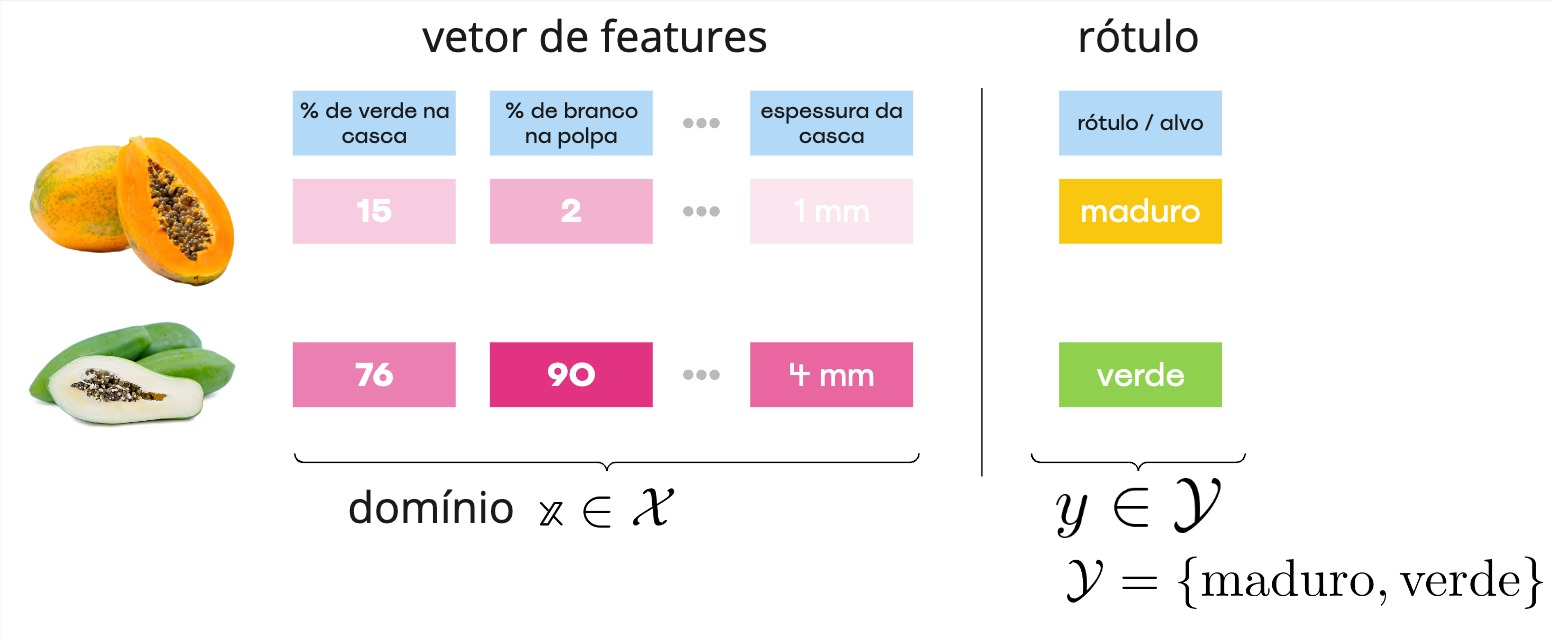
\includegraphics[width=0.8\paperwidth]{./imgs/fig8-papaya-scenario.jpg}
    \end{center}
\end{frame}


\begin{frame}
    \frametitle{Modelo formal de aprendizado}
    \begin{block}{Dados}
        Coletamos dados de muitas papaias colhidas no passado. Para cada uma criamos um \textbf{vetor de características} $\mathbb{x}\in\mathcal{X}$ e um \textbf{rótulo} $y\in\{\text{maduro}, \text{verde}\}$.
    \end{block}

    \begin{block}{Preditor}
        Queremos encontrar uma função que, para cada $\mathbb{x}$ , retorne uma previsão para o rótulo $y$: 
        $$h: \mathcal{X}\to\{\text{maduro}, \text{verde}\}$$
    \end{block}
\end{frame}

\begin{frame}
    \frametitle{Modelo formal de aprendizado}
    \begin{block}{Distribuição dos dados}
        Suponha que os dados coletados são descritos por uma distribuição de probabilidades $D$:
        $$(\mathbb{x}, y) \sim D$$
    \end{block}
    \begin{block}{Probabilidade de erro}
        Podemos avaliar o preditor pela probabilidade de que ele cometa um erro:
        $$\varepsilon[h] = \mathrm{Pr}_{(\mathbb{x}, y) \sim D}\left\{h(\mathbb{x})\neq y\right\}$$
        Um bom preditor tem esse erro o menor possível.
    \end{block}
    \begin{alertblock}{Problema}
        Não é possível calcular $\varepsilon[h]$ de antemão. Não conhecemos $D$!!!
    \end{alertblock}
\end{frame}

\begin{frame}
    \frametitle{Modelo formal de aprendizado}
    \begin{block}{Mas podemos coletar dados e aproximar $\varepsilon[h]$}
        Suponha que temos um monte de \textbf{exemplos} coletados:
        $$
            S = \left\{(\mathbb{x}_k, y_k)\sim D  \mid k =1, 2, \ldots, N\right\}
        $$
        
        Podemos fazer uma estimativa do \textbf{erro empírico}: 
        $$
            \hat\varepsilon_S[h] = \frac{1}{N}\sum_{k=1}^N \mathbb{1}\left[h(\mathbb{x}_k)\neq y_k\right]
        $$
        Dessa forma, um possível preditor "aprendido" através dos exemplos seria através da \textbf{minimização do erro empírico}.
        $$
            h^{\star} = \arg\min_{h \in \mathcal{H}}\hat\varepsilon[h]
        $$

    \end{block}
\end{frame}

\begin{frame}
    \frametitle{Problema: Generalização e Overfitting}
    \begin{block}{Suponha o seguinte preditor}
        $$
        h(\mathbb{x}) = \begin{cases}
            y_k,              & \text{if } \mathbb{x} = \mathbb{x}_k\\
            \mathrm{verde},   & \text{otherwise}
        \end{cases}
        $$
    \begin{center}
        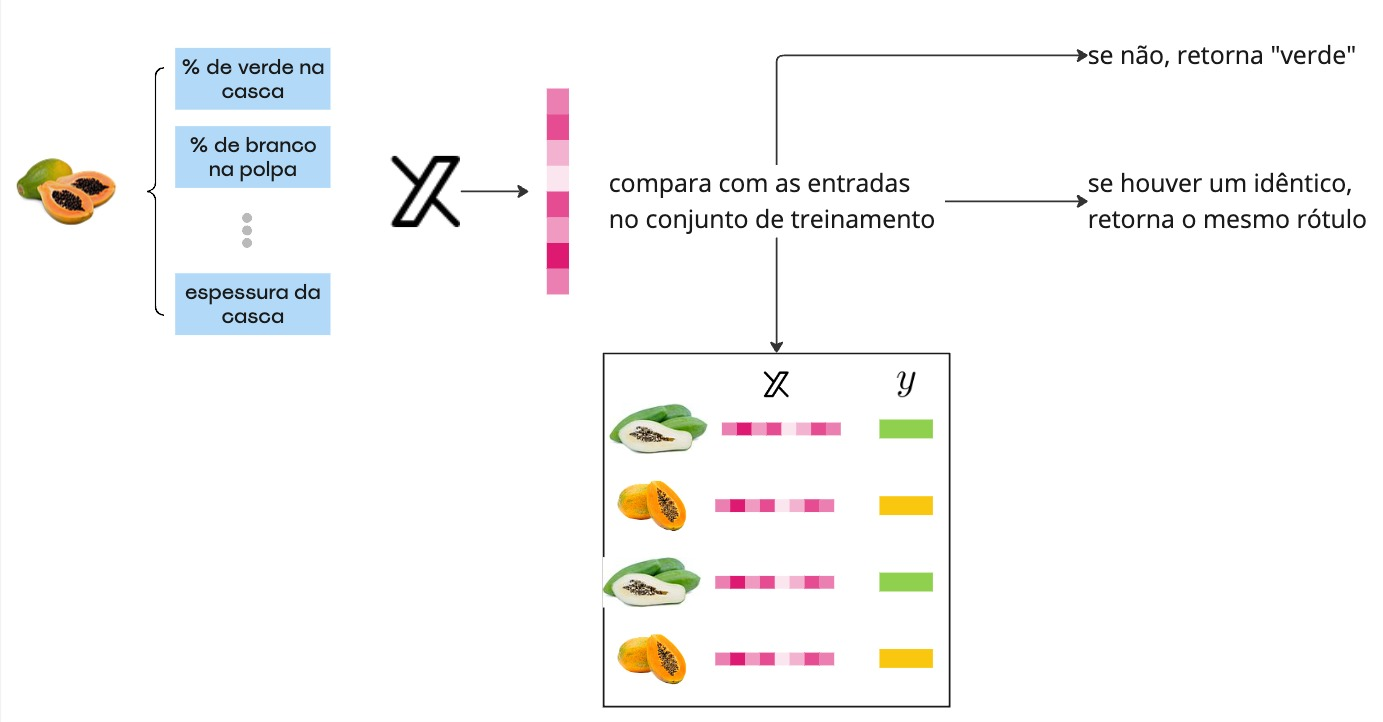
\includegraphics[width=0.65\paperwidth]{./imgs/fig9-preditor-trivial.jpg}
    \end{center}\vspace{-4mm}
    Qual é o erro empirico desse preditor?
    \end{block}
\end{frame}

\begin{frame}
    \frametitle{Problema: Generalização e Overfitting}
    \begin{block}{Suponha o seguinte preditor}
        $$
        h(\mathbb{x}) = \begin{cases}
            y_k,              & \text{if } \mathbb{x} = \mathbb{x}_k\\
            \mathrm{verde},   & \text{otherwise}
        \end{cases}
        $$
    O preditor tem erro empírico zero!!! Mas... é um bom preditor?
    \end{block}
    \begin{block}{Overfitting}
        O preditor não comete nenhum erro no conjunto de dados usado para treiná-lo, mas não é capaz de \textbf{generalizar} para novos casos. A resposta para qualquer novo caso é $\mathrm{verde}$.
    \end{block}
\end{frame}


\begin{frame}
    \frametitle{Erro de treinamento e erro de generalização}
    \begin{block}{}
    Para determinar quão bem um preditor é capaz de classificar nossas papaias, é importante que \textbf{o erro empírico seja calculado em um conjunto não usado para treiná-lo}!
    Definimos o conjunto de treinamento $T$ e o conjunto hold-out $H$ fazendo uma \textbf{partição aleatória} dos dados coletados em $S$.\footnote{Por exemplo, colocando um exemplo em $T$ com probabilidade 0.8 e em $H$ com probabilidade 0.2}

    Erro de treinamento:
    $$ \varepsilon_{\text{train}}[h] = \hat\varepsilon_T[h]  $$
    Erro de generalização:
    $$ \varepsilon_{\text{gen.}}[h] = \hat\varepsilon_H[h]  $$
    \end{block}
\end{frame}

\begin{frame}
    \frametitle{Dilema Viés-Variância}
    \begin{center}
        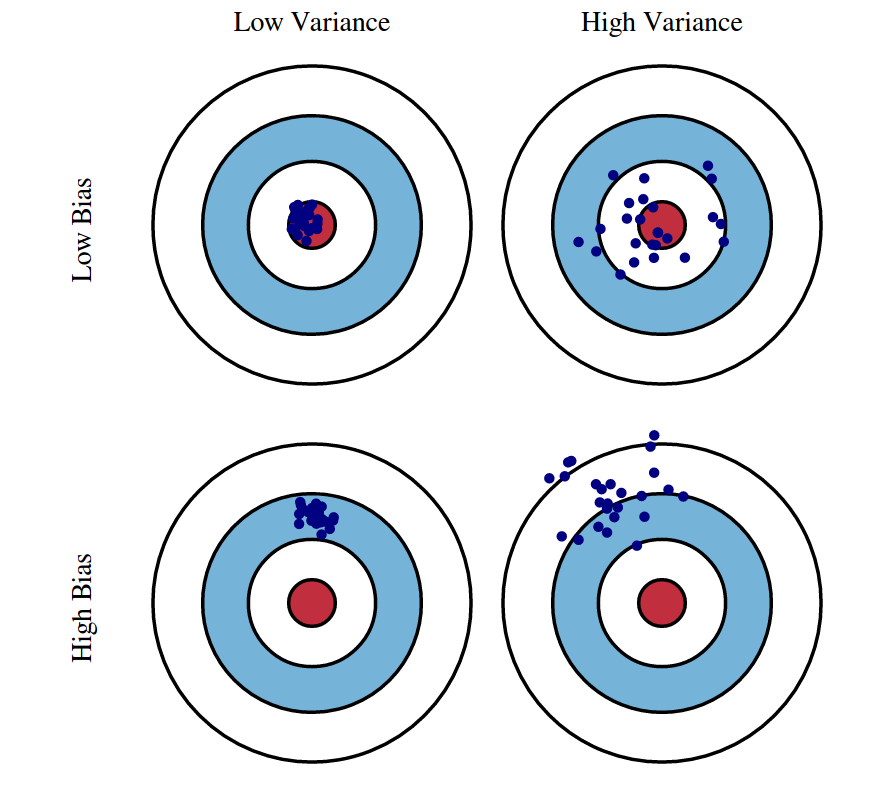
\includegraphics[width=0.55\paperwidth]{./imgs/fig10-bias-variance.png}
    \end{center}\end{frame}

\begin{frame}
    \frametitle{Dilema Viés-Variância}
    \begin{center}
        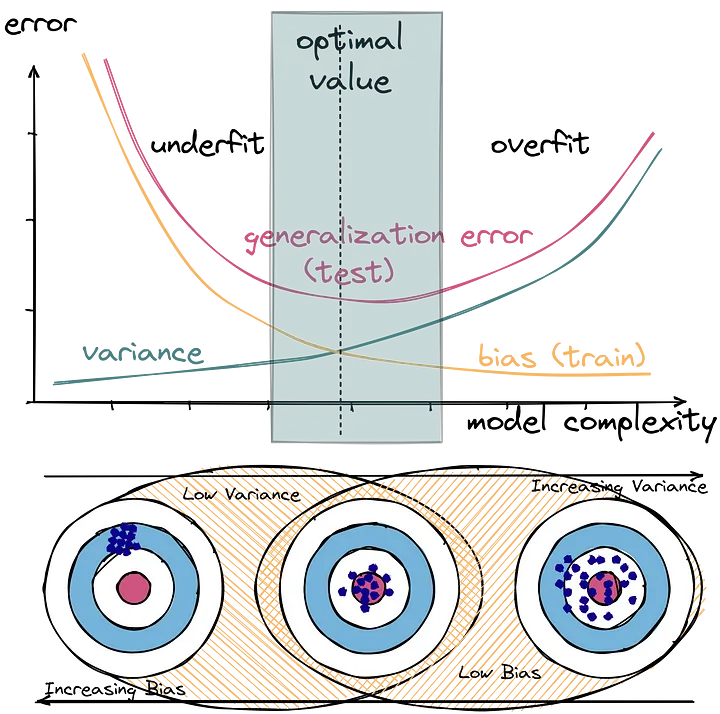
\includegraphics[width=0.55\paperwidth]{./imgs/fig11-bias-variance.png}
    \end{center}
\end{frame}


